\documentclass[FM,DP]{tulthesis}

% fonts, langs, packages...
\usepackage{polyglossia}
\setdefaultlanguage{czech}
\PolyglossiaSetup{czech}{indentfirst=true}
\usepackage{fontspec}
\usepackage{xunicode}
\usepackage{xltxtra}
\setsansfont[Mapping=tex-text,BoldFont={* Bold},Numbers=OldStyle]{Myriad Pro}
\usepackage{hyperref}
\hypersetup{colorlinks=true, linkcolor=tul, urlcolor=tul, citecolor=tul}
\usepackage{graphicx}
\usepackage{mathtools}
\usepackage{booktabs}
\usepackage{listings}
\usepackage[toc,page]{appendix}
\usepackage{amsmath}
\usepackage{amssymb}
\newcommand{\argument}[1]{{\ttfamily\color{\tulcolor}#1}}
\newcommand{\prikaz}[1]{\argument{\textbackslash #1}}
\newenvironment{myquote}{\begin{list}{}{\setlength\leftmargin\parindent}\item[]}{\end{list}}
\sloppy

\usepackage{array}
\newcolumntype{L}[1]{>{\raggedright\let\newline\\\arraybackslash\hspace{0pt}}m{#1}}
\newcolumntype{C}[1]{>{\centering\let\newline\\\arraybackslash\hspace{0pt}}m{#1}}
\newcolumntype{R}[1]{>{\raggedleft\let\newline\\\arraybackslash\hspace{0pt}}m{#1}}

% syntax highlighting
\usepackage[newfloat]{minted}
\usepackage[labelfont=bf,font=it]{caption}
\usepackage{etoolbox}
\definecolor{bg}{rgb}{0.95,0.95,0.95}
\setminted{bgcolor=bg, frame=single, rulecolor=\color{bg}, breaklines=true}
\makeatletter
\patchcmd{\minted@colorbg}{\noindent}{\medskip\noindent}{}{}
\apptocmd{\endminted@colorbg}{\par\medskip}{}{}
\makeatother
\newenvironment{code}
    {\filbreak\captionsetup{type=listing}}{\filbreak}
\SetupFloatingEnvironment{listing}{name=Výpis}
\renewcommand{\floatpagefraction}{.8}%

% brak lines in \url{}
\makeatletter
\g@addto@macro{\UrlBreaks}{\UrlOrds}
\makeatother

% toc
\renewcommand{\listlistingname}{Seznam výpisů programů}


%%%%%%%%%%%%%%%%%%%%%%%%%%%%
\begin{document}
\pagenumbering{gobble}

{\thispagestyle{empty}

\begin{center}
\bfseries
\LARGE
Vysok\'a \v skola ekonomick\'a v Praze\\ 
\vspace{3mm}
\Large
Fakulta informatiky a statistiky\\\vspace{1mm}
\vspace{1mm}
Katedra informa\v cn\'ich technologi\'i
\vspace{3cm}
\end{center}

\vfill

\begin{center}
\Huge\bfseries
DevOps -- konec zavedeným pořádkům vývoje a řízení kvality softwaru?
\par
\vspace{15mm}
\end{center}

\begin{center}
\Large\bfseries
\MakeUppercase{Semestrální práce}
\vspace{3cm}
\end{center}

\vfill

\list{}{\leftmargin=2.7cm}\item[]
\large\noindent\begin{tabularx}{\linewidth}{@{}lX@{}}
\color{tulgray}%
Předmět: & 4IT446 -- Řízení kvality softwaru \\
\color{tulgray}%
Student: & Bc. Luděk Veselý \\
\color{tulgray}%
E-mail: & vesl00@vse.cz \\
\end{tabularx}
\endlist
\list{}{\leftmargin=-3.1cm}\item[]
\endlist

\vfill

\begin{center}
\Large\bfseries
2017
\end{center}

\vspace*{-1cm}
\cleardoublepage}


%%%%%%%%%%%%%%%%%%%%%%%%%%%%
\pagenumbering{roman}
\setcounter{page}{2}
\addcontentsline{toc}{chapter}{Obsah}
\tableofcontents
\clearpage

%% obrazky
%\addcontentsline{toc}{chapter}{Seznam obrázků}
%\listoffigures
%\clearpage
%
%% tabulky
%\addcontentsline{toc}{chapter}{Seznam tabulek}
%\listoftables
%\clearpage
%
%% vypisy programu
%\addcontentsline{toc}{chapter}{Seznam výpisů programů}
%\listoflistings
%\clearpage


%%%%%%%%%%%%%%%%%%%%%%%%%%%%
\pagenumbering{arabic}

\chapter{Úvod}

Vývoj software prošel za svou dobu řadou změn, stále jsou však využívány přístupy, které vznikly v době, 
kdy byly požadavky na vývoj jiné než v současné době. Nyní je vývoj software rychlejší a dynamičtější, je třeba
být schopen rychle reagovat na změny, umět doručit novou funkcionalitu uživateli co nejdříve. IT odvětví se
totiž odlišuje od odvětví tradičních, k řízení je tedy třeba přistupovat jinak, než v~případě tradičních odvětví.
Přestože se i v~rámci IT dílčí zaměření dosti odlišují (například požadavky na stabilitu systému jsou
jiné u zdravotnického zařízení a jiné u webové fotogalerie), stále se toto odvětví od~těch tradičních odlišuje.

Těmto problémům by měl pomoci čelit agilní přístup, který definuje jiné uvažování o vývoji software. Zákazník 
je v~samém centru dění a primární je jeho spokojenost. S tím také souvisí pojem DevOps, který popisuje propojení 
světů vývojářů, správců a testerů a vede tak k~odstranění bariér, které mohou blokovat uvedení software 
do~provozu.

\begin{figure}[h]
\center

\includegraphics[width=\textwidth]{devops.png}
\caption{Vztah vývoje, provozu, QA a DevOps (Zdroj: \cite{devops-img})}
\label{devops}
\end{figure}

Tato práce si klade za cíl provést světem DevOps -- vysvětlit, proč může být přínosné tento koncept adoptovat
a představit technické prostředky, kterými lze tohoto cíle dosáhnout. Cílem této práce není popisovat, 
co to vlastně DevOps je nebo jaká je jeho historie. Tato práce je spíše praktický průvodce, který čtenáři dodá 
přehled technik a nástrojů, které mu pomohou v adaptaci tohoto přístupu.

V úvodu práce je vysvětlen stav, kdy je aplikace implementována jako jeden celistvý systém a o~její provoz
se stará někdo jiný, než ji vyvíjí, což s~sebou nese řadu problémů, zejména co se zodpovědnosti
týče. Následně je zavedena filozofie DevOps, a vysvětleno, jak může pomoci čelit zmíněným problémům. 
Následně jsou popisovány vybrané prostředky pomáhající v~naplnění DevOps ideálů -- architektura mikroslužeb, 
kontinuální integrace a nasazování, kontejnerizace, monitoring.


\chapter{DevOps jako nový přístup k řízení vývoje a kvality software}

Za dobu vývoje a řízení kvality software se procesy s tím související ustálily. Jednotlivé role
nebo pozice v IT světě jsou obecně známé včetně náplně jejich práce a souvisejících kompetencí. 
Jenže tento přístup je praktikován již nějakou dobu a v okamžiku svého vzniku rozhodně nebylo počítáno
s bouřlivostí a rychlostí rozvoje IT, jak ji známe dnes. Stále častěji se tak mluví o DevOps jako
nástupci zavedených pořádků v řízení vývoje a kvality software. Než bude vysvětleno, v~čem tento
přístup spočívá, je žádoucí krátce vysvětlit, v~čem spočívá tradiční přístup k vývoji a jaká jsou jeho
úskalí.

\section{Tradiční způsob vývoje aplikací}

Tradiční způsob řízení vývoje software vycházející z vodopádového modelu se přenáší i na způsob
jeho nasazování do produkčního prostředí. Vývojáři (\textbf{Developers}) programují kód, který je
třeba pro potřeby testování a akceptace zpřístupnit tak, aby byl veřejně dostupný pro danou skupinu 
uživatelů (testerů nebo zadavatelů). Typicky tak vzniká několik prostředí (vývojové, testovací, 
produkční nebo akceptační), v~nichž je aplikace nasazena v~různých verzích a konfiguracích, s~různými daty. 
To s~sebou nese problém správy jednotlivých prostředí a následného nasazování aplikace do těchto prostředí.
Je to tak prostor pro vznik chyb, navíc je potřeba pracovník (nebo jejich skupina), který se
o tato prostředí bude starat -- těmto lidem se souhrnně říká \textbf{Operations}.

\begin{figure}[h]
\center
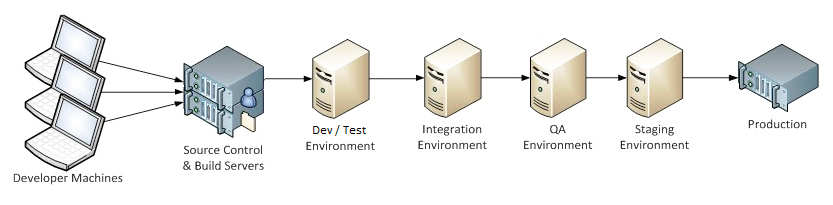
\includegraphics[width=\textwidth]{deployment.png}
\caption{Řada prostředí pro manuální schválení software (Zdroj: \cite{deployment})}
\label{deployment}
\end{figure}

Tento přístup má samozřejmě řadu důvodů, proč je využíván. V prvé řadě se každé činnosti věnuje
specialista v daném oboru. Provozu aplikace se věnuje pracovník, který se může zabývat pouze
touto prací a nemusí se zaobírat programováním, může se ve svém oboru více specializovat.

Dále má každý vývojář vždy k dispozici kompletní aplikaci, nemusí tak zprovozňovat více prostředí pro 
vývoj. Nemusí se ani starat o provoz testovacího prostředí, zjednodušeně řečeno pouze naprogramuje
a odevzdá, co je po něm požadováno.

Zároveň je pomocí tohoto přístupu možné dosáhnout pořádku v nasazování v tom smyslu, že je dostatečně 
dlouhá doba do nasazení změny a při dodržení definovaných procesů je taková změna důsledně testována
při jejím schvalování. Přestože se zdá, že takový systém musí bez problémů fungovat, v~praxi může být
situace jiná. Požadavky na změnu mohou být velmi časté s nutností jejich rychlého zapracování.


\section{Problémy vyskytující se u tradičního přístupu}

Tento přístup k nasazování aplikací se však potýká s řadou problémů. Vzhledem k oddělení prostředí
trvá velmi dlouho, než se naprogramovaná změna dostane do~produkčního prostředí. Na této cestě
je příliš mnoho překážek, jako jsou jednotlivá schvalování a ruční zásahy. Díky tomu zadavatel vidí
funkční artefakt až příliš pozdě a musí si tak umět včas představit, co by měl vyvíjený software
umět, což je v případě IT projektů nesmírně obtížné \cite[strana~73]{devops}.

\begin{figure}[h]
\center
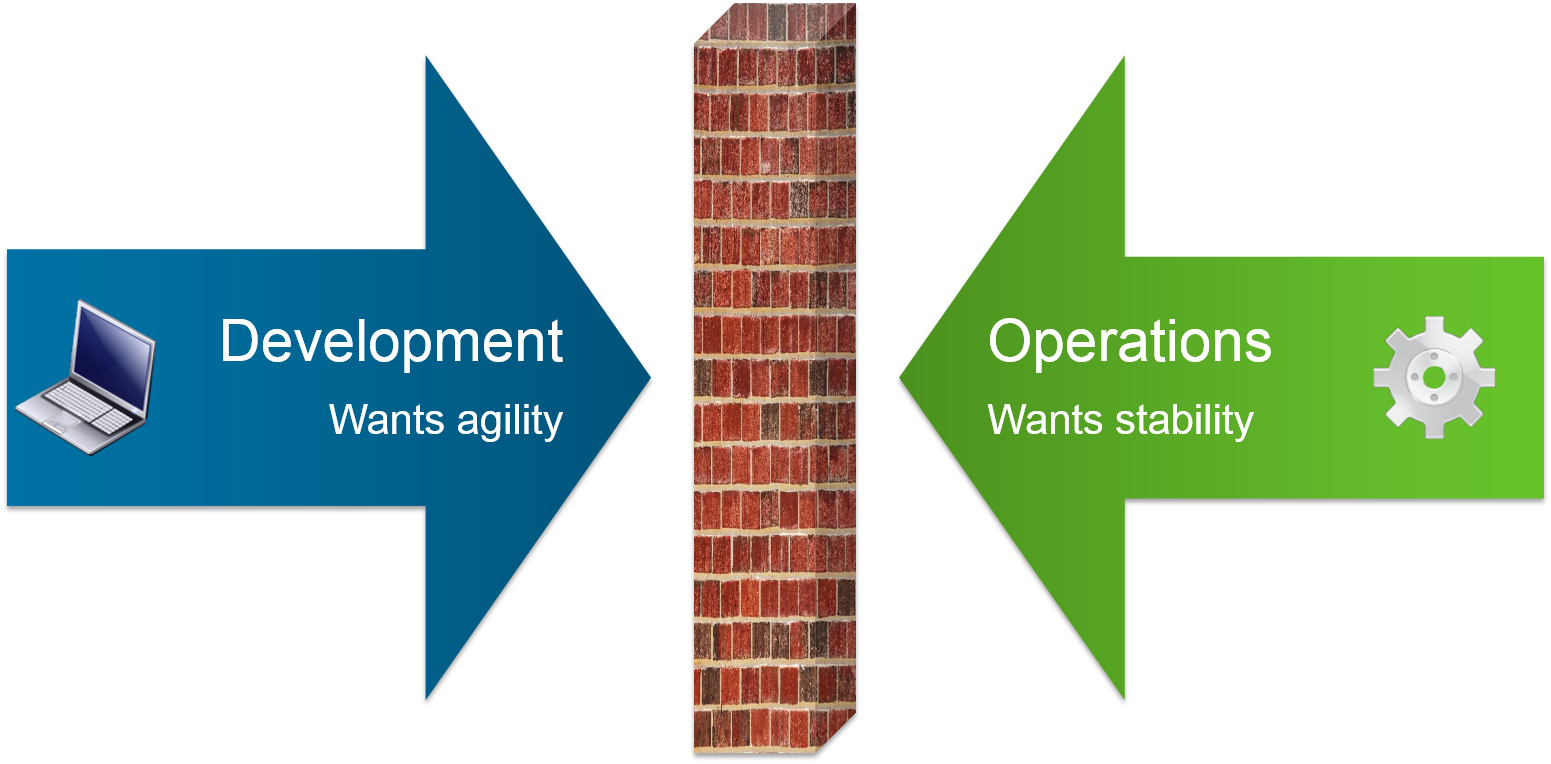
\includegraphics[width=\textwidth]{devops-wall.png}
\caption{Bariéra mezi vývojovým a provozním týmem (Zdroj: \cite{devops-wall})}
\label{devops-wall}
\end{figure}

Dále zde vzniká problém se zodpovědností za odvedenou práci, kdy programátoři chtějí co nejčastěji
nasazovat své změny, naproti tomu provozní tým se snaží zachovat stabilitu a co nejvyšší dostupnost
služby, což jsou protichůdné požadavky. V~nejhorším případě si lze takovou situaci představit 
jako zeď, přes kterou je kód přehazován, což je znázorněno na obrázku \ref{devops-wall}.
Pokud nastane v aplikaci chyba, může být obtížné identifikovat jejího autora, což vede k následnému
upřesňování předávky kódu aplikace mezi týmy a k dalšímu zesložiťování celého procesu nasazování.

Pokud nejsou jednotlivé kroky při nasazování aplikace automatizovány, je problém rychlost jejich provádění
a samozřejmě je také třeba počítat se zvýšeným rizikem vzniku chyb. 

\section{Propojení vývoje a provozu -- DevOps}

Pro čelení těmto problémům vznikla filozofie DevOps, jež si dává za cíl oba světy (vývoj i provoz) propojit.
DevOps je primárně o kultuře -- pokud není ve firmě zájem jej zavádět, je jeho použití prakticky nemožné. Týmy
by měly být otevřené a chtít sdílet znalosti, spolupracovat na řešení problémů, být připraveni nést odpovědnost.
K tomu je nutné počítat se zavedením automatizace a samozřejmě také měřit vhodné metriky pro ověření dosaženého
zlepšení. DevOps je na rozdíl od Tradičního přístupu kontinuální proces, který se neustále opakuje.

\begin{figure}[h]
\center
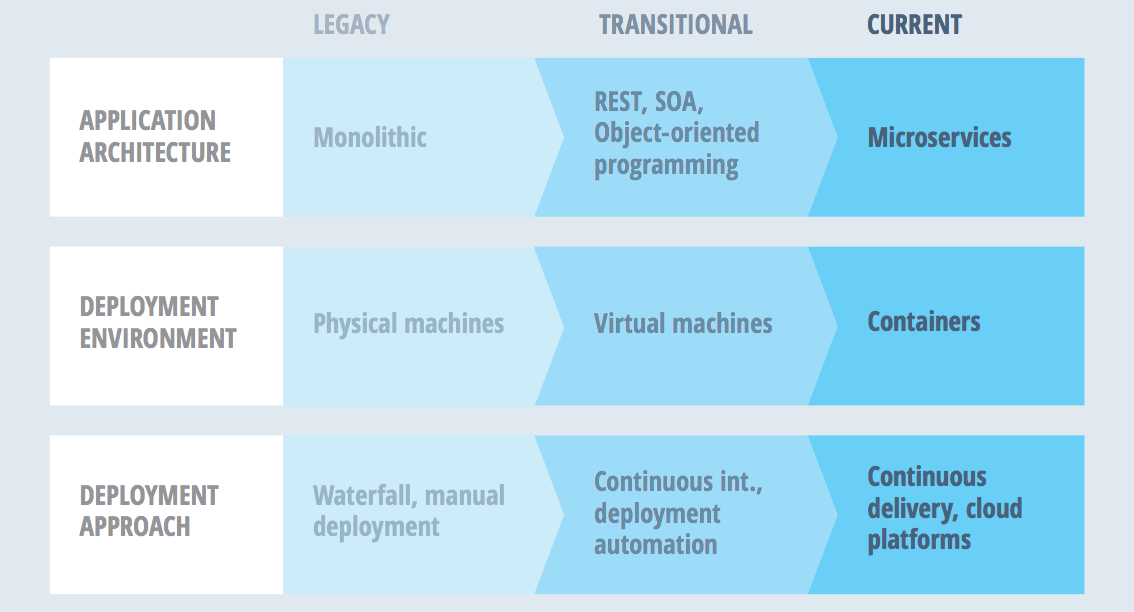
\includegraphics[width=\textwidth]{devops-vs-traditional.png}
\caption{Vývoj architektury a nasazování software (Zdroj: \cite[strana~109]{microservices})}
\label{devops-vs-traditional}
\end{figure}

Vzhledem k rozsahu této práce se z~výše uvedeného dále zabývám jen zaváděním automatizace -- nelze pokrýt veškerá 
témata dostatečně 
podrobně. Filozofie DevOps postupně promlouvá do přístupu k~návrhu architektury software a způsobu provozu a
nasazování software. Namísto monolitické architektury nabývá na popularitě architektura mikroslužeb, software
je dodáván častěji po menších změnách a plně automatizovaně, což je znázorněno na obrázku \ref{devops-vs-traditional}.

V této práci uvedené principy a techniky naleznou nejlepší uplatnění při vývoji a dodávce software poskytovaného
jako služba. Je zřejmé, že některé druhy software buď není možné nebo naopak není žádoucí dodávat kontinuálně,
agilním způsobem. Prvním příkladem může být software v kávovaru, ke~kterému nemá vývojář po jeho prodeji přístup, 
druhým příkladem budiž software autonomního řízení vozidla, které musí procházet zcela odlišnými schvalovacími
procesy.

\chapter{Prostředky DevOps}

Pro dosažení ideálu DevOps je kromě samotné změny přemýšlení nad dodávkou software také nutné se zamyslet
nad technickými prostředky. Pokud je vyvíjená aplikace velká a její nasazení trvá příliš dlouhou dobu, 
je adaptace agilního přístupu téměř nemožná, protože samotné nasazení aplikace veškerou agilitu pohřbí.
Je na místě přemýšlet o tom, jak změny doručovat častěji, po menších částech, až kontinuálně. Jako vhodné
se jeví změna architektury tak, aby bylo možné nasazovat častěji a automatizace běžných a opakujících se
činností v průběhu integrace změn a jejich doručování.

\section{Architektura mikroslužeb}

Jako první je při adaptaci konceptu DevOps nutné přizpůsobit architekturu samotné aplikace. Cílem
je umožnění častého nasazování, což je problém v situaci, kdy je třeba sestavit a otestovat komplexní
aplikaci.

\begin{figure}[h]
\center
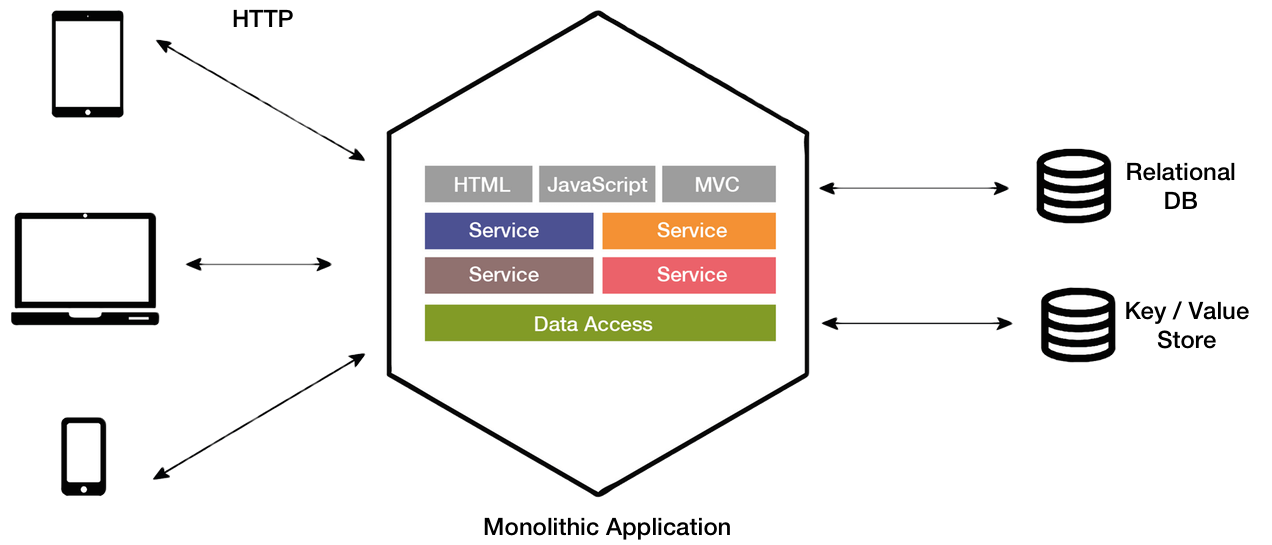
\includegraphics[width=\textwidth]{monolith.png}
\caption{Monolit (Zdroj: \cite{monolith})}
\label{monolith}
\end{figure}

Uvažujme elektronický obchod, který je implementován jako jedna celistvá aplikace, která umožňuje
zákazníkům nakupovat, zákaznické podpoře pracovat s objednávkami, účetním pracovat s fakturami
a zároveň také vedení firmy generovat reporty. Pokud by v~tomto případě bylo třeba provést triviální 
opravu v~jedné části aplikace, je nutné ji vždy otestovat a nasadit celou. Samozřejmě by bylo možné
testovat pouze tu část aplikace, které se změna týká, není pak ale možné odhalit, zda případná chyba
neovlivní úplně jinou část aplikace \cite[strana~77]{devops}. V~takovou chvíli je třeba se rozhodnout, do~jaké 
míry je třeba aplikaci testovat, zda případně není možné počkat, až bude nasaditelných změn více. V~tento 
okamžik ale může být možnost pružně reagovat na požadavky obchodu dokonce i konkurenční výhodou.
Problémem takové aplikace je také možnost jejího škálování. V okamžiku, kdy není možné navyšovat
výkon stroje, na kterém je provozována (vertikální škálování), je možné škálovat horizontálně pouze 
přidáváním dalších instancí celé aplikace, přestože je fakticky třeba navýšit výpočetní kapacitu pouze 
pro jednu konkrétní část aplikace \cite[strana~78]{devops}.

Způsob návrhu, kdy jsou spolu všechny části aplikace provázány a musí být nasazovány společně se
nazývá \textbf{monolitická architektura} \cite[strana~7]{microservices}. V praxi bych tento návrh architektury 
použil pouze u projektu, který je malý (co do množství zdrojového kódu) a nepředpokládá se u něj v~budoucnu 
další výrazné rozšiřování. Další podmínkou pro jeho úspěšné použití by byla práce jediného programátora na~celém 
projektu. Jinak docházelo spíše k odkládání nasazení a následným obavám, zda se něco nerozbije, protože případná
oprava by trvala příliš dlouho. Dalším důsledkem byl problém aktualizace vývojových nástrojů a prostředí, 
v~nichž aplikace běží, což by znamenalo výpadek celé aplikace. V případě, že se neaktualizovalo zase vzrůstalo
riziko odhalení bezpečnostních chyb a v konečném důsledku byl také problém nalézt vývojáře, kteří jsou ochotni
pracovat s neaktuálními technologiemi.

\begin{figure}[h]
\center
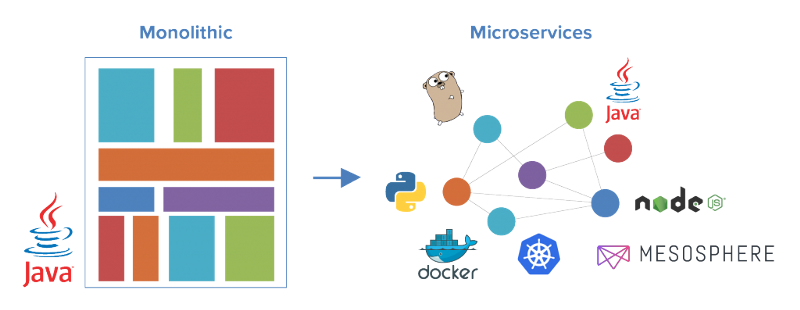
\includegraphics[width=\textwidth]{monolit-vs-microservices.png}
\caption{Rozdíl mezi monolitickou architekturou a mikroslužbami (Zdroj: \cite{microservices-blog})}
\label{monolit-vs-microservices}
\end{figure}

Naproti tomu \textbf{architektura mikroslužeb} umožňuje rozdělení aplikace na několik samostatných celků.
Každý díl (mikroslužba) je samostatná aplikace, která je samostatně nasaditelná a spustitelná a disponuje
vlastním rozhraním, kterým s~ní lze komunikovat \cite[strana~8]{microservices}. Konkrétním příkladem na případu
elektronického obchodu je rozdělení na službu obsluhující objednávky, dále službu obsluhující produkty a tak dále. 
Primární výhodou tohoto přístupu je jednoduchost a samostatnost každé mikroslužby. Díky tomu, že řeší jeden izolovaný 
problém, je pro programátora snadnější ji pochopit a udržovat, je možné ji daleko rychleji otestovat a nasadit. 
Dále je také možné pro její vývoj zvolit optimální technologie -- pro ukládání objednávek bude vhodné
použít databázi, která zajistí především bezpečné uložení dat, naproti tomu pro službu zobrazující produkty bude 
vhodnější použít databázi, která nabízí rychlé čtení a dostatek funkcí pro textové vyhledávání \cite[strana~83]{devops}.

\subsection{Velikost mikroslužeb}

Zde je třeba se pozastavit a rozhodnout, jak velké mají mikroslužby být, což je hojně diskutovaný problém 
\cite[strana~13]{microservices}. Pokud jsou příliš malé a je jich příliš mnoho, může to v konečném důsledku 
přinést spíše problémy. Provoz každé služby totiž obnáší určitou režii, kterou je třeba brát v~potaz. Typicky 
má každá služba vlastní repozitář, vlastní konfigurace a další závislosti. Na druhou stranu však příliš malé 
služby nemusí dosáhnout kýženého přínosu. Je také třeba přemýšlet o možném budoucím škálování služeb. Obecně 
lze aplikace škálovat třemi způsoby: použitím mikroslužeb, jejich duplikací a shardováním databáze, což je
znázorněno na obrázku \ref{microservices-scale}. V~praxi se mi osvědčila dvě pravidla, která mohou poukázat 
na~optimální velikost služby, případně na způsob jejich návrhu.

\begin{figure}[h]
\center
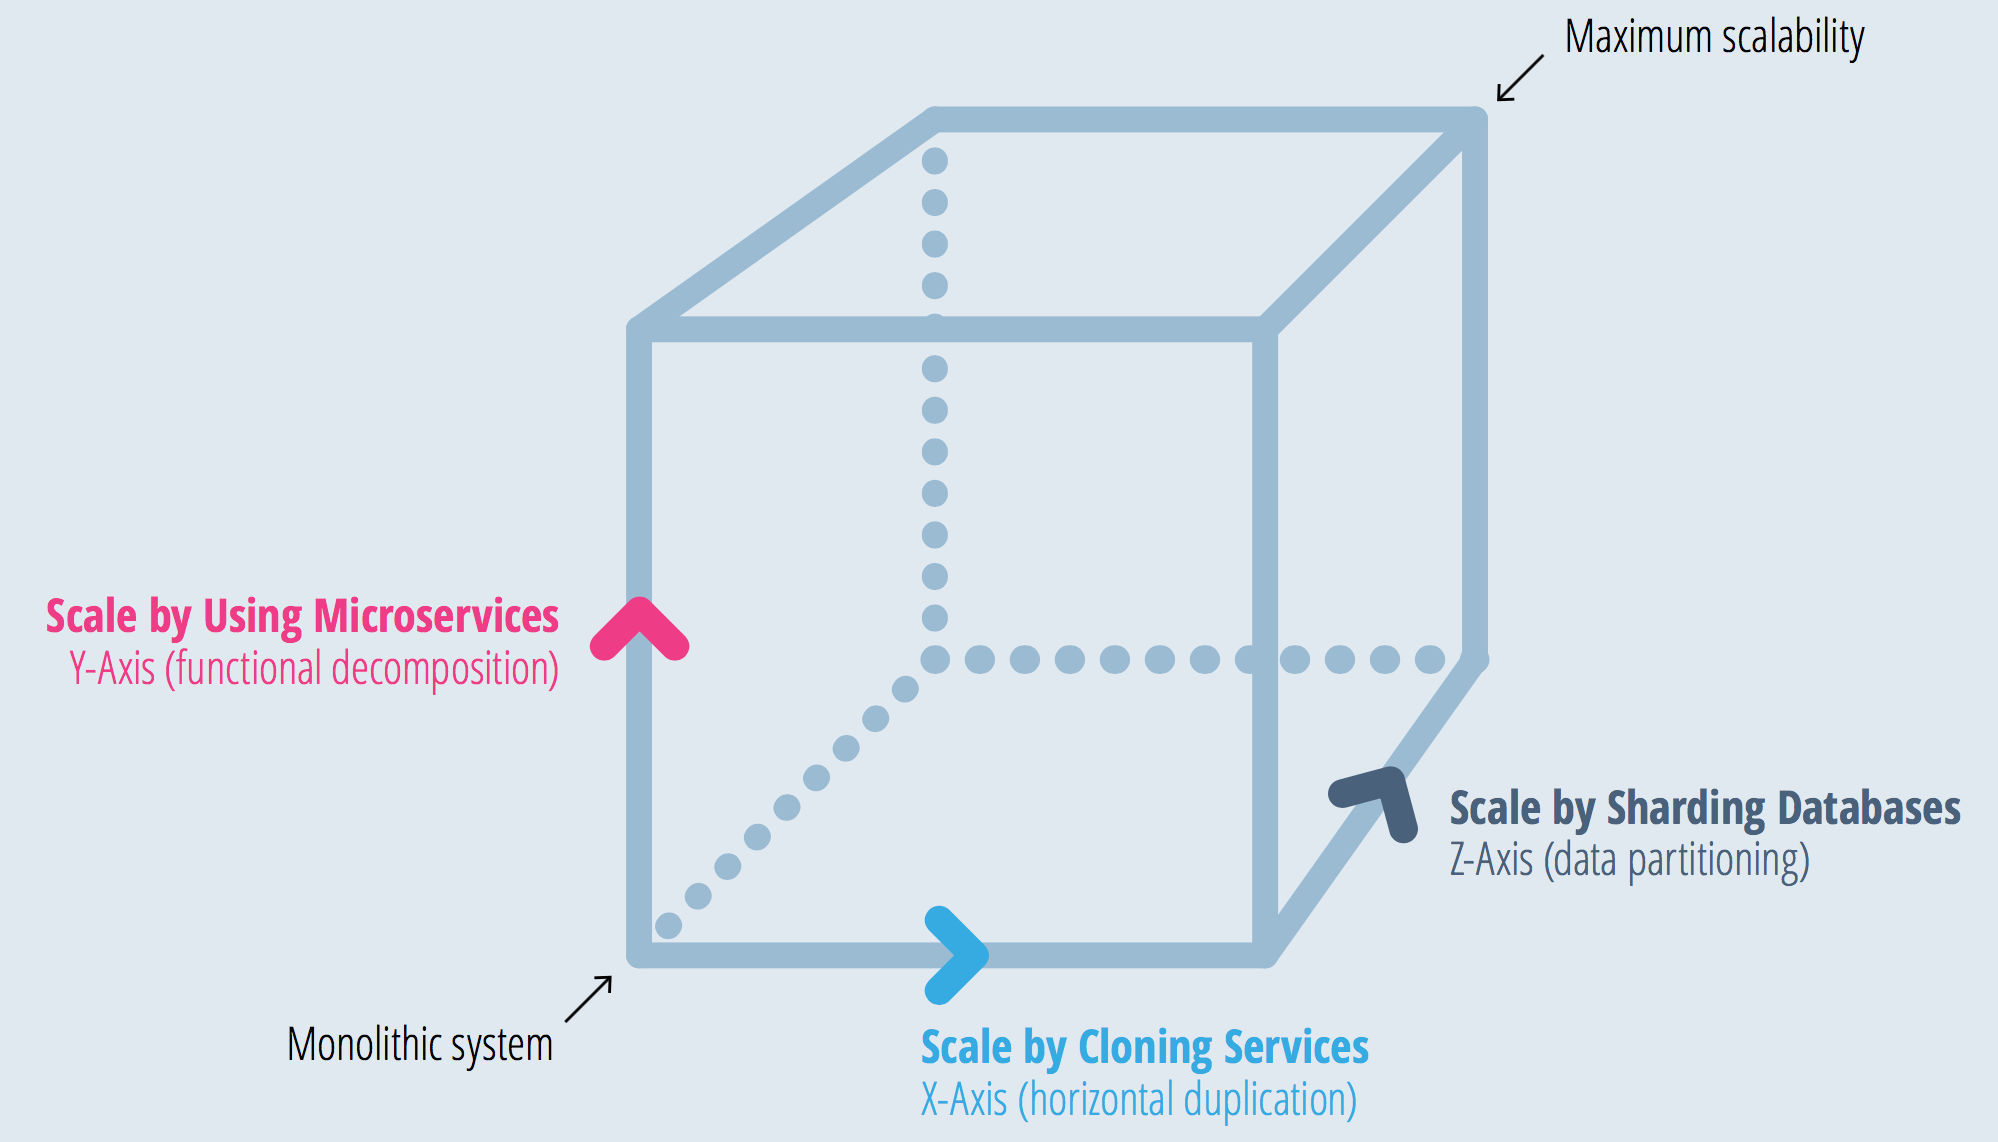
\includegraphics[width=\textwidth]{microservices-scale.png}
\caption{Dimenze škálování a mikroslužby (Zdroj: \cite[strana~10]{microservices})}
\label{microservices-scale}
\end{figure}

Prvně lze začít vyčleňováním samostatně funkčních celků. Je třeba identifikovat vhodné kandidáty, v případě e-shopu
to může být například systém pro rozesílání novinek elektronickou poštou. Následně lze postupně oddělovat další
části, které mohou být samostatně funkční. Ve výsledku jsou tak mikroslužby děleny dle logických částí
aplikace, tak jak mají na starosti jinou část obchodu \cite[strana~11]{microservices}. Tento postup je 
spíše dlouhodobý, osvědčil se mi ale v případě, kdy byla aplikace technologicky zastaralá a její další rozšiřování
(nebo jen aktualizace) je problematické.

Rozdělení aplikace na služby lze vztáhnout i k rozdělení týmů nebo lidí ve firmě. Pokud se jeden vývojář stará v~rámci 
e-shopu o~vyhledávání produktů, nabízí se, aby právě vyhledávání bylo implementováno jako jedna služba s jasně 
definovaným rozhraním. Pokud pak tento vývojář potřebuje načíst informace o počtu prodaných kusů daného produktu, 
provede to voláním služby zastřešující objednávky -- obdobně, jako by se ptal kolegy, který se o~tuto oblast stará.
Struktura služeb tak kopíruje strukturu firmy. K tomuto poznání často dojdou firmy samy, aniž by si to uvědomovaly, 
myšlenka je to však stará padesát let a je známá jako Conway's Law~\cite{monolith}.

\subsection{Problémy při implementaci mikroslužeb}

V okamžiku, kdy přibývají další mikroslužby lze pozorovat, že se v určitých rysech shodují. Často využívají
stejné vývojové nebo běhové prostředí, pracují s~obdobnými zdroji. To může vést ke snaze opakující se činnosti
nějakým způsobem standardizovat nebo vyčleňovat \cite[strana~24]{microservices}. Ať už se jedná o vytváření 
sdílených knihoven  nebo standardizaci rozhraní a chování služeb, je to krok zpět, který degraduje 
využití potenciálu mikroslužeb a zavádění inovací do firmy \cite[strana~27]{devops}.

Nelze také opomenout to, že problémy, které existují při vývoji monolitických aplikací se objevují také
u mikroslužeb, avšak na vyšší úrovni \cite{microservices-blog}. Pokud je špatně navržena funkce a ta je 
volána mnohokrát, je to jisté zdržení v provádění kódu. V případě mikroslužeb je však takové zdržení 
mnohonásobně delší, protože spolu služby komunikují po síti prostřednictvím definovaného protokolu, 
což je řádově náročnější, než prosté volání funkce.


\section{Kontinuální integrace a nasazování}
\label{section:ci}

V této kapitole jsou popsány kroky, vedoucí k automatizaci testování a nasazování software. To je důležité
pro to, aby byly vytvořené změny co nejdříve dostupné ostatním vývojářům a uživatelům. Nelze však pouze povolit
všem veškeré pravomoci k nasazování software, je třeba dodržet několik pravidel, aby byl tento proces spolehlivý
a přínosný.

\begin{figure}[h]
\center
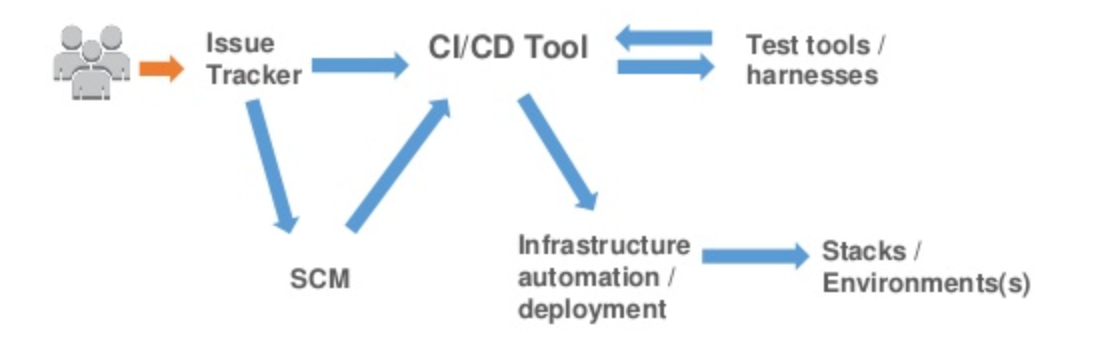
\includegraphics[width=\textwidth]{ci-cd-pipeline.png}
\caption{Průběh kontinuálního nasazování (Zdroj: \cite{ci-cd-pipeline})}
\label{ci-cd-pipeline}
\end{figure}

Nejprve je třeba si ujasnit základní pojmy související s kontinuální integrací \cite{ci}. V praxi se používají 
následující tři pojmy (bývají však často zaměňovány, nebo souhrnně označovány jako CI/CD, podrobnější popis
rozdílů je například v~\cite{ci-cd}):

\begin{itemize}
\item \textbf{Kontinuální integrace} (continuous integration): Kód je několikrát denně ukládán 
do~centrálního repozitáře a je prováděna kontrola tohoto kódu
\item \textbf{Kontinuální doručování} (continuous delivery): Navíc k integraci je sestaven artefakt, 
který je nasaditelný
\item \textbf{Kontinuální nasazování} (continuous deployment): navíc k doručování je tento artefakt 
nasazen do provozu
\end{itemize}

Postup integrace je zpravidla následující: Uživatel nahraje změny v~zdrojových kódech do sdíleného repozitáře, 
ten oznámí integračnímu nástroji detail této změny. Integrační nástroj zkontroluje zdrojový kód a pokud je 
v~pořádku, vytvoří artefakt, který je možné nasadit. Posledním krokem je samotné nasazení vytvořeného artefaktu 
do~provozu, přičemž o~celém průběhu je vývojář průběžně informován.

\subsection{Nástroje pro kontinuální integraci}

Nástrojů, které umožňují kontinuální integraci je celá řada, jejich komplexní výčet je k~dispozici 
v~\cite[strana~139]{microservices}. Výběr vhodného nástroje je závislý na požadavcích a možnostech dané
společnosti. Základní členění je podle toho, zda je daný nástroj poskytován jako služba, nebo si jej
musí uživatel spravovat sám. Každé řešení má své výhody a nevýhody, každý podnik je schopný akceptovat
něco jiného, obecně však je viditelná tendence firem spíše využívat služeb. Dalším kritériem
výběru je otevřenost nástroje a jeho cena. Konečně je také kritériem pro výběr nástroje jeho
funkčnost, rychlost implementace a podpora napojení na další systémy.

\begin{figure}[h]
\center
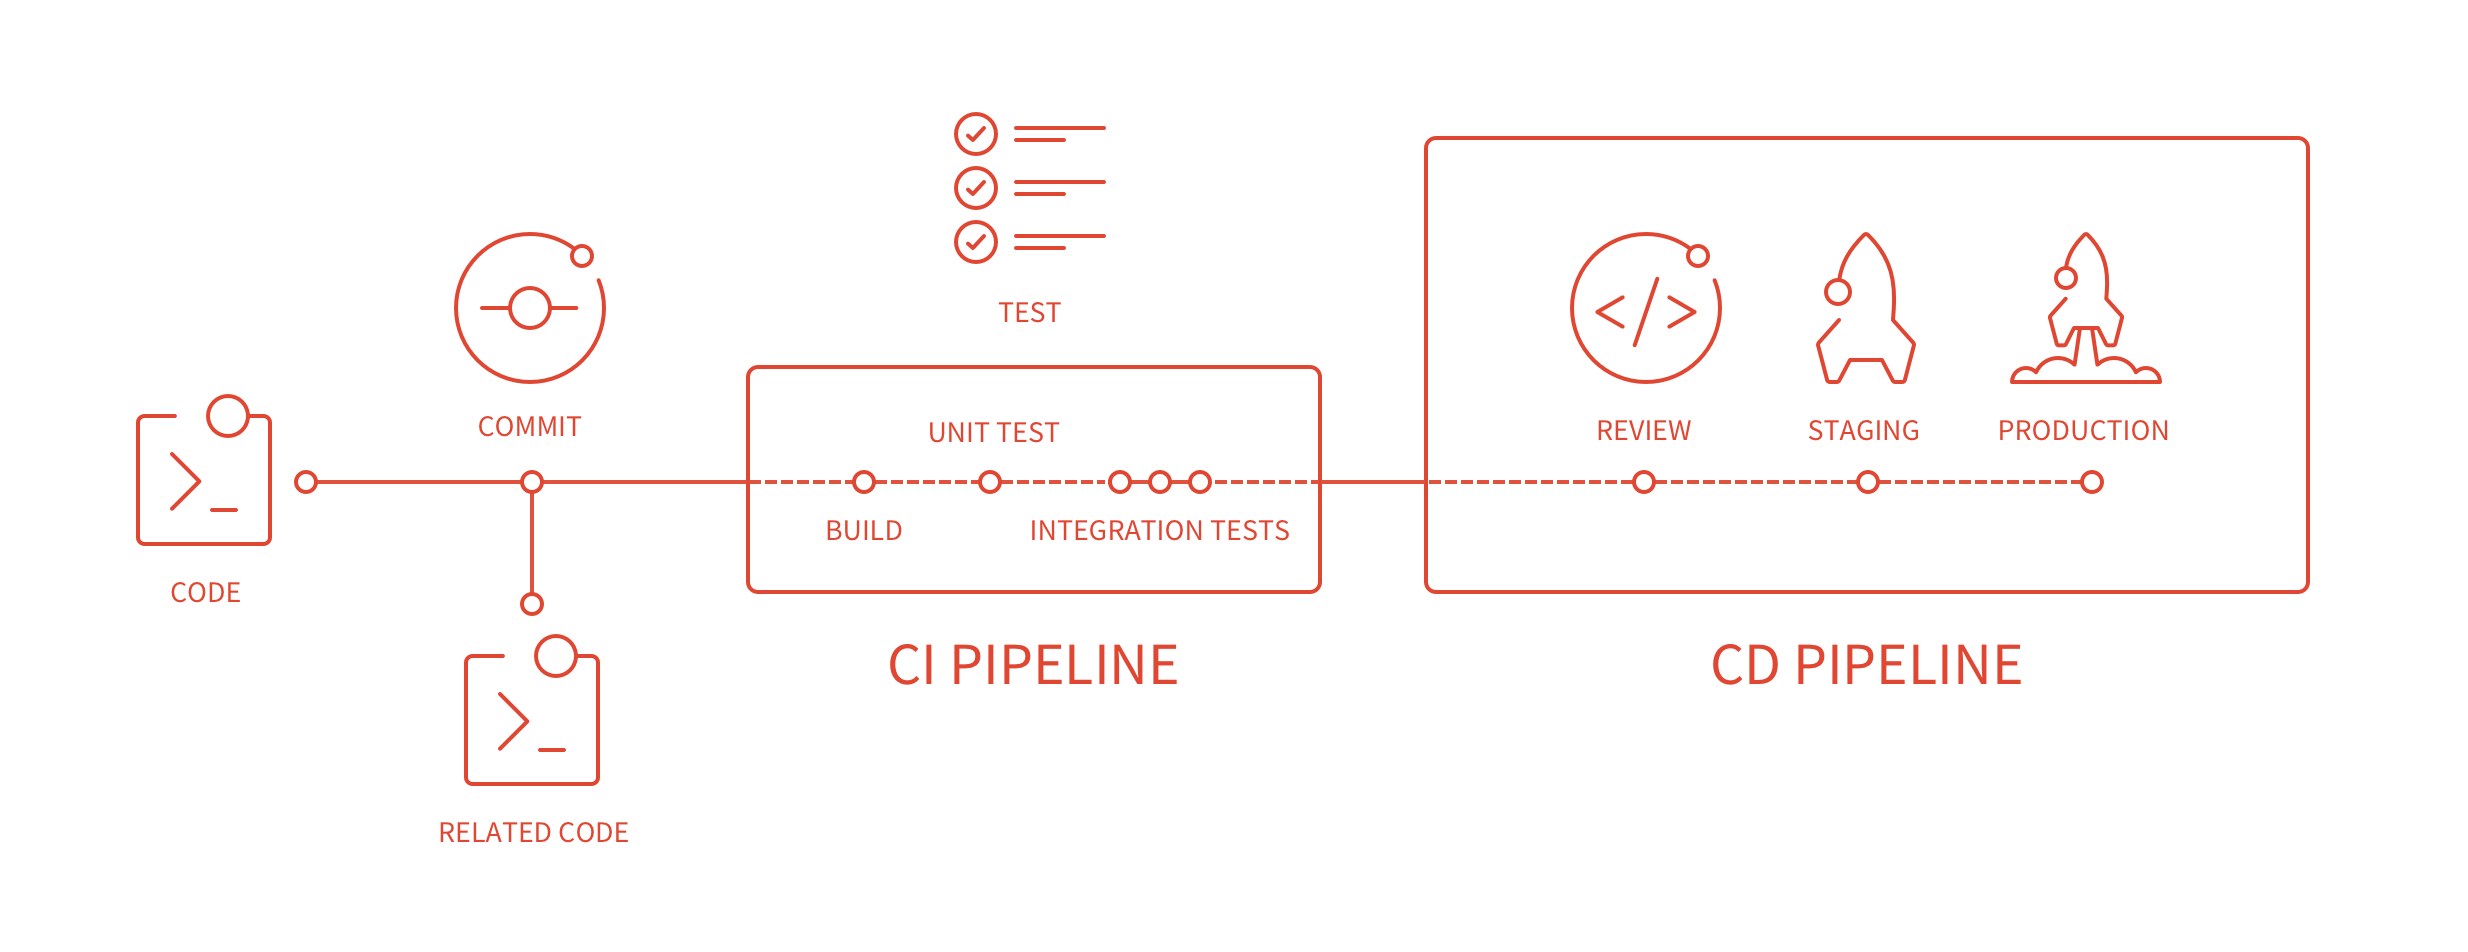
\includegraphics[width=\textwidth]{ci-steps.png}
\caption{Dílčí kroky integračního serveru (Zdroj: \cite{gitlab})}
\label{ci-steps}
\end{figure}

V praxi jsem používal více nástrojů - GitLab CI, CircleCI, Drone, Jenkins a Bamboo. Z těchto nástrojů je
jediný kompletně placený nástroj Bamboo \cite{bamboo}, který byl použit z~důvodu dostupné integrace s~dalšími 
nástroji firmy Atlassian. Bohužel tento nástroj optimálně nepodporuje agilní přístup a tak celý proces 
zpomaluje. Zajímavý je nástroj Drone \cite{drone}, který je extrémně štíhlý a rychlý, dostupný včetně zdrojových kódů. 
Jeho nevýhodou může být nutnost jej zprovoznit a spravovat na své vlastní infrastruktuře, na druhou stranu ale 
nedisponuje žádnými omezeními, může tak jít při častějším používání o cenově výhodnější řešení. Na stejném
principu je k dispozici Jenkins \cite{jenkins}, který je jedním z nejrozšířenějších nástrojů v oboru. Populární
je zejména díky dostupné řadě pluginů, které umožňují nástroj přizpůsobit téměř jakýmkoli potřebám. Je však třeba
počítat s vyšší složitostí, zejména ve srovnání s Drone. Naproti tomu CircleCI \cite{circle} je poskytován jako služba,
přičemž je možné provádět souběžně právě jednu integraci, další navyšování výpočetní kapacity je zpoplatněno. 
Výhodou této služby je řada předinstalovaných a předkonfigurovaných nástrojů, které lze použít. Automaticky
je tak možné detekovat například použitý framework pro spuštění testů. Posledním nástrojem je GitLab CI \cite{gitlab},
který je dostupný všemi možnými způsoby - jako Open Source, jako placený, hostovaný i jako služba. Vzhledem k~jeho
dostupnosti a snadnosti použití budu dále uvádět ukázky právě pro GitLab CI.

\subsection{Implementace kontinuální integrace pomocí GitLab CI}

Základem je definovat jednotlivé kroky, které má integrační server vykonat. Ty jsou zpravidla rozděleny do fází
(stages), které seskupují příkazy zajišťující jeden druh činnosti. Může jít o instalaci závislostí, 
provedení statické analýzy, spuštění jednotlivých testů (jednotkových, integračních, zátěžových...), vytvoření
artefaktu, jeho zveřejnění a následné nasazení do odpovídajícího prostředí, případně otestování po tomto nasazení --
tyto fáze jsou znázorněny na obrázku \ref{ci-steps}. Následně jsou v~rámci těchto sekcí prováděny jednotlivé
příkazy, kterými může být konkrétní spuštění skriptu, programu nebo utility.

\begin{figure}[h]
\center
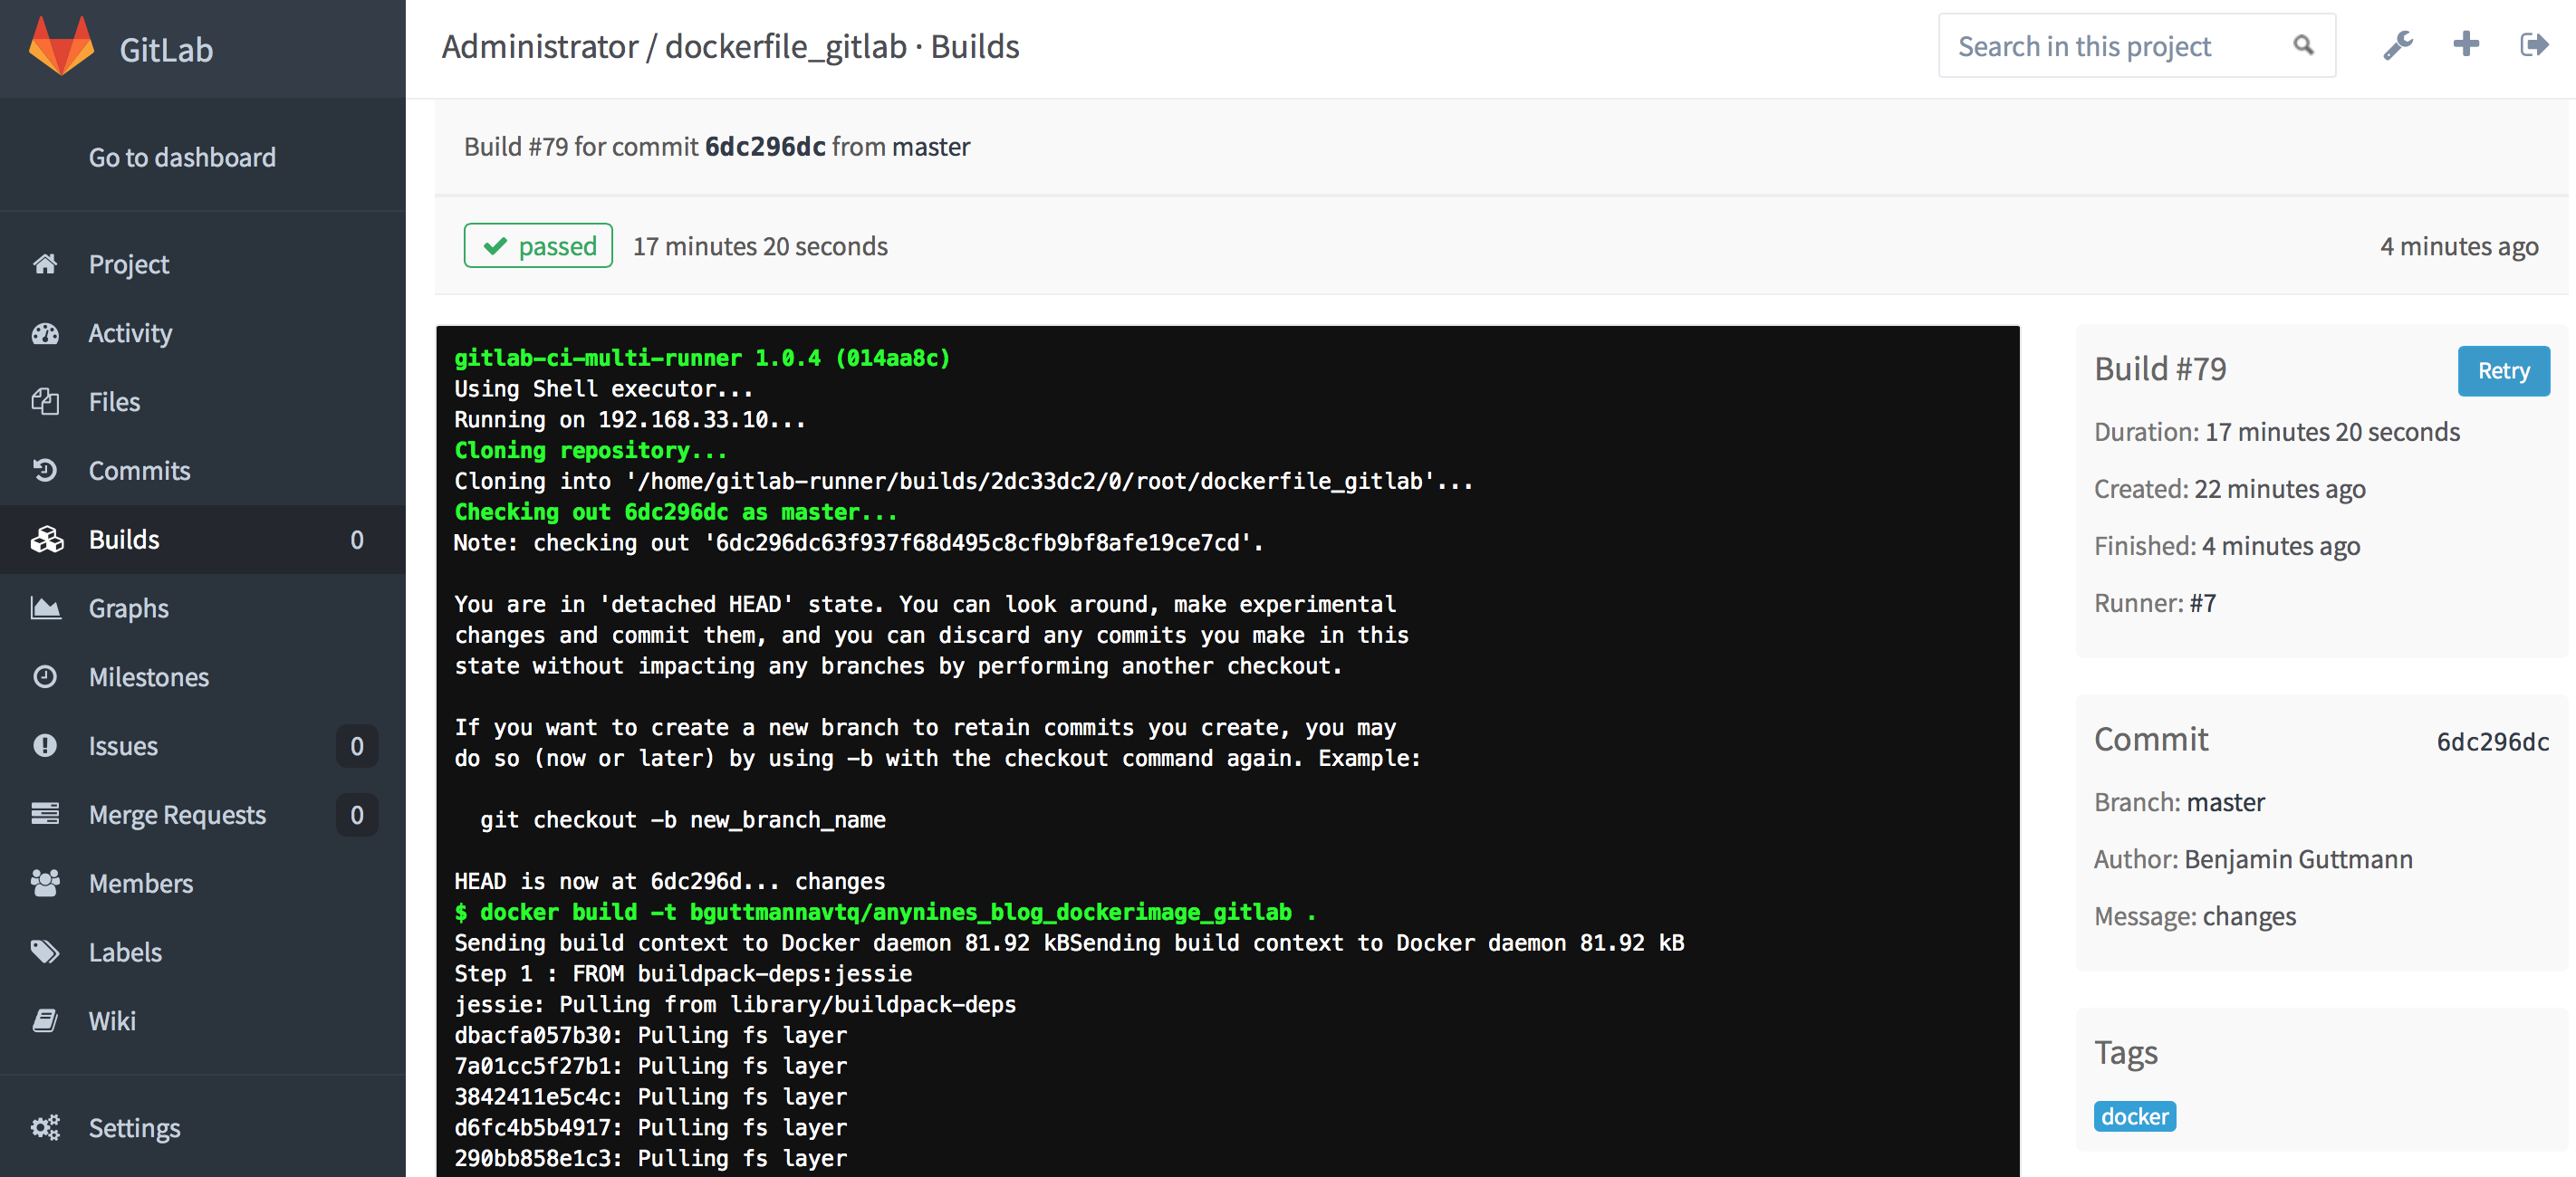
\includegraphics[width=\textwidth]{gitlab.png}
\caption{Sledování průběhu integrace v GitLab CI (Zdroj: \cite{gitlab})}
\label{gitlab}
\end{figure}

Například konfigurace pro projekt psaný v jazyce PHP, který je třeba sestavit, otestovat, zveřejnit a nasadit
by vypadala následovně: nejprve by bylo v souboru \verb|.gitlab-ci.yml| třeba definovat sekce, kterými je třeba
projít v sekci \verb|stages|. Následně jsou pro každou sekci uvedeny příkazy, které se mají vykonat -- pokud je
daná sekce vykonána úspěšně (příkazy končí návratovým kódem \verb|0|), postupuje se ve vykonávání k~další sekci.
Kupříkladu druhá sekce má na starosti spuštění testů, přičemž nejprve je provedena statická analýza kódu pomocí
nástroje \verb|phpcs|, následně jsou spuštěny jednotkové testy nástrojem \verb|phpunit| a nakonec také akceptační
nebo integrační pomocí nástroje \verb|codeception|, který na pozadí spouští webový prohlížeč. Celá konfigurace
je zobrazena ve výpisu \ref{code:gitlab}, přičemž dále popisuje stažení závislostí a sestavení balíčku v sekci 
\verb|build|, jeho zveřejnění v sekci \verb|release| a nakonec také nasazení v sekci \verb|deploy|.

Jediným limitem je zde nutnost použití integrace současně s repozitářem GitLab. Ten je nabízen zdarma jako služba
a s~integrační částí sdílí společné grafické rozhraní. Přímo v~kódu je tak vidět, co již bylo
integrováno a s~jakým výsledkem. Průběh integrace může sledovat každý, kdo má k~repozitáři přístup, 
na obrázku \ref{gitlab} lze vidět průběh právě probíhající integrace. Vhodné je také provést propojení
s~chatem (například Slack nebo HipChat) -- poté je v případě neúspěchu ihned jasné, kdo celou
pipeline rozbil a může se tak ihned začít pracovat na nápravě. 

\begin{code}
\captionsetup{singlelinecheck=false,justification=raggedright}
\captionof{listing}{Ukázková konfigurace pro GitLab CI}
\label{code:gitlab}
\begin{minted}{yaml}
stages:
    - build
    - test
    - release
    - deploy
build:
    stage: build
    script:
        - composer install
        - docker build -t my-app .
test:
    stage: test
    script:
        - vendor/bin/phpcs
        - vendor/bin/phpunit
        - vendor/bin/codeception run
release:
    stage: release
    script:
        - docker push my-app
deploy:
    stage: deploy
    script:
        - kubectl apply -f kube-config.yaml
\end{minted}
\end{code}

Adaptace kontinuální integrace je pro mě v dnešní době automatická a je to většinou první krok po vytvoření
repozitáře pro sdílení zdrojových kódů. Sice jde o práci navíc, zrychlení dalšího vývoje ale investovaný čas 
navrátí. Navíc je mnohem snazší nastavit přísné kontroly kódu u nového projektu, než u projektů existujících.

U již rozběhlých projektů je implementace složitější, zejména pokud
je cílem zavést kontrolu kódu tam, kde v minulosti nebyla prováděna. V tomto případě se mi osvědčilo 
zavést určitou hranici (například počet tolerovaných chyb mess detektoru) s~tím, že se nesmí zvyšovat
a o~volných chvílích se nabízí práce na snížení této hranice. Jako důležité také shledávám možnost konfigurace
integračního nástroje souborem, který je součástí zdrojových kódů -- díky tomu jsou mohou být veškeré změny 
v~konfiguraci schvalovány a verzovány.

\section{Kontejnerizace}

S mikroslužbami a kontinuální integrací souvisí také to, že je třeba nějakým způsobem vytvořit takový artefakt, 
který bude možné snadno distribuovat a spustit. K~tomu by bylo možné vytvářet binární soubory, JAR nebo DLL
balíčky, nicméně ne každý programovací jazyk toto umožňuje -- například skriptovací jazyky zpravidla
vyžadují nějaké běhové prostředí. To není úplně ideální situace ve chvíli, kdy pracujeme s mikroslužbami, 
a s každou z nich se pracuje jinak, což komplikuje jejich provoz. 

\begin{figure}[h]
\center
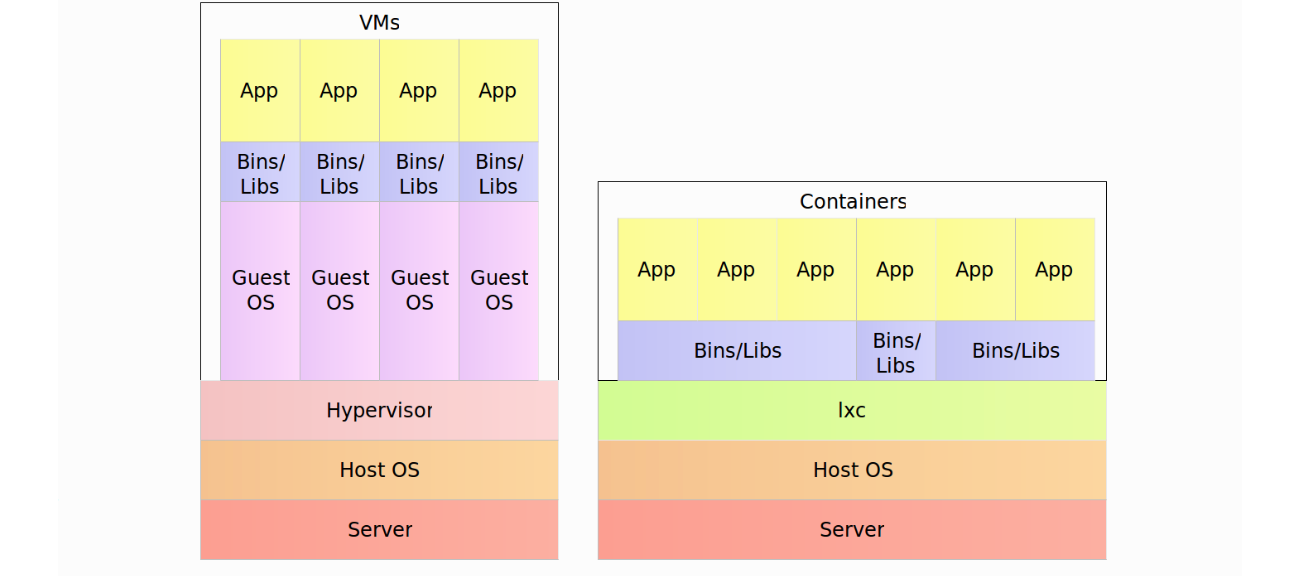
\includegraphics[width=\textwidth]{container-vs-vm.png}
\caption{Porovnání virtálního stroje a kontejneru (Zdroj: \cite[strana~68]{devops})}
\label{container-vs-vm}
\end{figure}

Pro zefektivnění provozu je přínosné vycházet z~metodologie The Twelve-Factor App~\cite{12factor}, 
která přináší sadu doporučení, jak těmto problémům čelit. Tato doporučení lze shrnout do několika bodů:

\begin{itemize}
\item Používání deklarativního formátu pro veškeré nastavení -- nemělo by být nutné cokoliv ručně konfigurovat
veškeré konfigurační soubory by měly být součástí kódu (stejně jako příklad konfigurace GitLab CI v~kapitole
\ref{section:ci}).
\item Jasně definovat rozhraní, kterým je možné se spustitelnými balíčky pracovat -- ať už jde o~jejich spouštění
a ovládání, monitoring nebo nastavení.
\item Minimalizaci rozdílů pro spouštění v~různých prostředích včetně cloudu, s~čímž souvisí připravenost
pro~bezproblémové škálování.
\end{itemize}

\subsection{Docker}

Tomuto přístupu jde naproti použití kontejnerů. Ty jsou k~dispozici již řadu let, jejich popularizaci však
způsobil až Docker \cite{docker}, s~jehož pomocí je práce s kontejnery snadná. Kontejner si lze představit jako 
virtuální stroj, který obsahuje spouštěnou aplikaci se všemi jejími závislostmi, který je však snadné distribuovat 
a spouštět. Přesnější je však o~kontejneru mluvit jako o izolovaném procesu, což lépe vystihuje jeho rychlost
spouštění a výkonnost, protože kontejner sdílí řadu prostředků s~operačním systémem, v~němž je spouštěn.

\begin{figure}[h]
\center
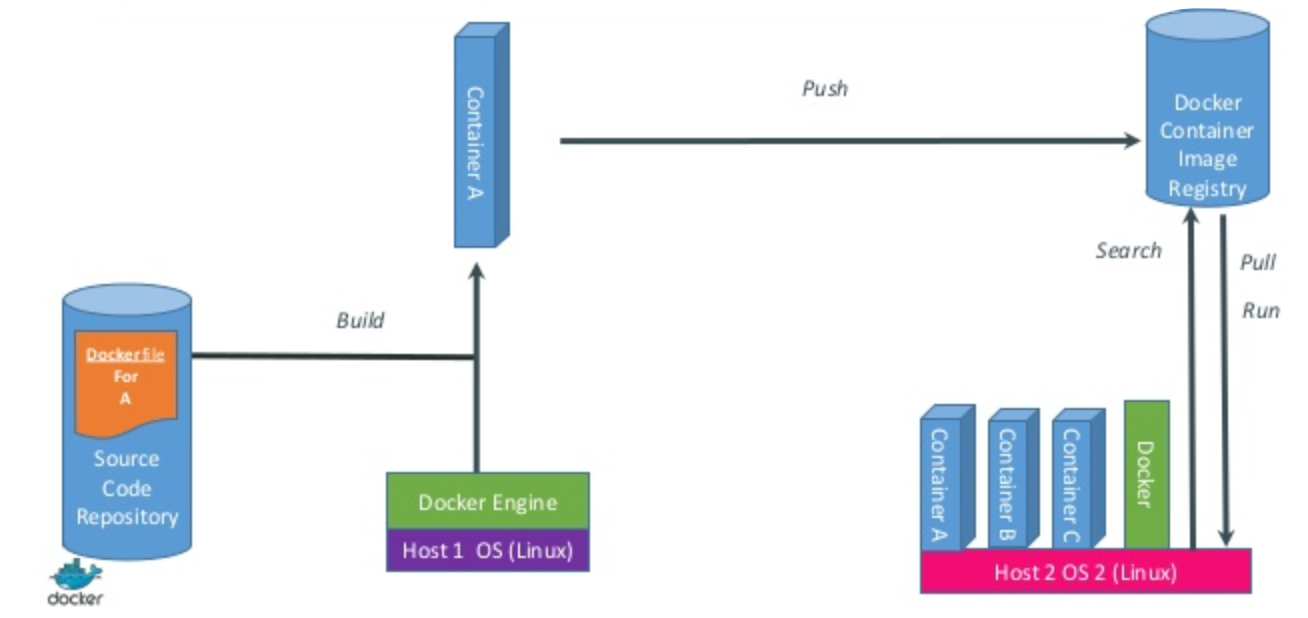
\includegraphics[width=\textwidth]{docker-flow.png}
\caption{Kroky při práci s nástrojem Docker (Zdroj: \cite{docker-flow})}
\label{docker-flow}
\end{figure}

Práce s nástrojem Docker probíhá následovně: Nejprve je napsán \verb|Dockerfile| (příklad je ve výpisu
\ref{code:dockerfile}), což je soubor, který definuje kroky, kterými vzniká tzv. obraz (Docker image). Prvním 
krokem je zpravidla zvolení základního obrazu, z~kterého se vychází. To může být jak štíhlá linuxová distribuce typu 
Busybox, tak kompletní distribuce jako Debian nebo CentOS. Přestože se může zdát vhodné použít známou plnohodnotnou
distribuci obsahující všechny myslitelné nástroje, je daleko vhodnější použít co nejjednodušší distribuci. Jednak se 
tím sníží požadavky na~propustnost sítě a velikost diskového prostoru a s~obrazy je tak možné lépe manipulovat (rychleji 
je distribuovat a spouštět), především je však zvýšena bezpečnost díky použití pouze nutných závislostí. Sestavit obraz 
je možné pomocí příkazu \verb|docker build -t my-app| spouštěném ve~složce obsahující \verb|Dockerfile|. Po~provedení 
tohoto příkazu je vytvořen obraz pojmenovaný jako \verb|my-app|. Ten je možné příkazem \verb|docker push my-app| 
nahrát do~veřejného úložiště, kterému se říká Docker Registry, přičemž pokud není řečeno jinak, tak je použito 
výchozí dostupné na~\url{https://hub.docker.com}. Na serveru je možné tento obraz spustit (a vytvořit tak kontejner)
příkazem \verb|docker run my-app|. Ten, pokud obraz nenalezne lokálně, stáhne obraz z~registru.

\begin{code}
\captionsetup{singlelinecheck=false,justification=raggedright}
\captionof{listing}{Příklad souboru Dockerfile}
\label{code:dockerfile}
\begin{minted}{docker}
# Volba základního obrazu - linuxové distribuce Alpine Linux
FROM alpine:3.1.0

# Instalace NGINX (webserver a proxy)
RUN apk --update add nginx

# Kontejner zveřejní port 80
EXPOSE 80

# Při spuštění kontejneru je spuštěn NGINX na popředí
ENTRYPOINT nginx -t
\end{minted}
\end{code}

Bylo by samozřejmě možné vzniklý obraz nahrát rovnou na server a tam ho spustit -- výhodou použití registru je však
to, že obraz může být stažen kdykoli i na jiný server, striktně tento přístup odděluje krok zveřejnění artefaktu
od kroku jeho nasazení. Dále jsou aplikace v kontejnerech nastavovány pomocí proměnných prostředí, mají přesně 
definované zveřejněné porty, produkují log jako proud událostí, což ctí principy \textit{The Twelve Factor Apps}. 
Největší výhodou kontejnerů je však to, že umožňují dosáhnout totožného prostředí pro běh aplikace bez závislosti 
na použitém stroji. Díky tomu lze předejít chybám, kdy se aplikace chovala korektně v testovacím prostředí ale ne 
v~produkčním, protože se zapomnělo na aktualizaci jedné knihovny. Dále značně zjednodušují lokální vývoj -- vzhledem 
k~nezávislosti na operačním systému, v němž jsou provozovány je schopen vývojář zprovozni prostředí pro vývoj během 
okamžiku. Po dokončení vývoje pouhým odstraněním stažených obrazů může uvést svůj stroj do stavu před stažením 
veškerých závislostí.

Docker sám o sobě však neřeší veškeré problémy, které se vyskytují při použití mikroslužeb a kontejnerů v~produkčním
prostředí. V praxi je třeba řešit také dostupnost aplikace, monitorovat a vyhodnocovat její chování, což je součástí
cyklu DevOps. S rostoucím množstvím provozovaných služeb a serverů je třeba řídit jejich provoz. Ve světě kontejnerů
se nástroje umožňující správu kontejnerů označují jako orchestrátory, přičemž jich existuje celá řada~\cite[strana~123]{orchestration}. Ty umožňují nasazení kontejnerů napříč celými clustery, kontrolu stavu jednotlivých kontejnerů, 
jejich dostupnost. Dokáží se tak vyrovnat se~selháním některého z serverů nebo škálovat konkrétní mikroslužbu při
jejím přetížení. Zároveň také umožňují agregaci logů, které kontejnery produkují a jejich zpřístupnění správci.


%%%%%%%%%%%%%%%%%%%%%%%%%%%%
\chapter{Závěr}

V této práci byly popsány problémy vznikající při vývoji a provozu software tradičním způsobem vycházejícím
z~vodopádového modelu. Byl zaveden pojem~DevOps, který přináší nový přístup k vývoji a provozu software, který
přináší otevřenost a zodpovědnost do těchto procesů, přičemž cílem je dodávání software tak, aby byl zákazník
spokojenější. Toho je dosahováno jak změnou kultury a uvažováním vývojářů a správců, tak zavedením řady technických
opatření nebo nástrojů.

Práce popisuje především technickou stránku zavádění DevOps, zaměřuje se na automatizaci procesů sovisejících
s nasazováním software. Podrobně je popsána architektura mikroslužeb, která umožňuje s aplikací pracovat 
prostřednictvím menších částí. Dále jsou popsány kontinuální integrace a nasazování jako způsob neustálého
automatického doručování software do produkčního prostředí. Nakonec jsou také popsány kontejnery jako způsob
efektivní distribuce jednotlivých služeb.

Vzhledem k rozsahu práce nebyla vyčerpána veškerá témata související s automatizací, ani nebyla všechna témata
probrána do dostatečné hloubky -- pro další prozkoumání problematiky lze doporučit literaturu uvedenou v~závěru
práce, zejména knihu The DevOps 2.0 Toolkit \cite{devops} a knihy z série The New Stack (\cite{microservices} a 
\cite{orchestration}). 

Z~témat, kterým by bylo vhodné se dále podrobněji věnovat je jistě orchestrace
(práce s vysokou dostupností aplikace) nebo monitoring (agregace logů, jejich vyhodnocování a alerting).
Jako teoretického nástupce kontejnerů pak lze v určitých případech uvést architekturu Serverless \cite{serverless},
která vývojáře plně odstiňuje od procesu sestavování balíčků nebo kontejnerů, ale je distribuován pouze kód, 
který je následně spouštěn pouze na infrastruktuře poskytovatele. Díky tomu není třeba při návrhu infrastruktury
uvažovat nad výkonností jednotlivých serverů a době jejich použití - v případě Serverless je infrastruktura
poskytovatele využita maximálně efektivně a zpoplatněna pouze za její faktické využití.


%%%%%%%%%%%%%%%%%%%%%%%%%%%%
\appendix
\begin{thebibliography}{Mm99} \addcontentsline{toc}{chapter}{Literatura}

% devops

\bibitem{devops} 
FARCIC Viktor. 
\emph{The DevOps 2.0 Toolkit: Automating the Continuous Deployment Pipeline with Containerized Microservices}. 
Packt Publishing, 2016 462~s. ISBN 978-1-78528-031-3.

\bibitem{devops-img}
SCHAEFFER Chuck. 
\emph{DevOps \& CRM Software Come Together} [online]. 
2017 [vid. 2017-05-01]. Dostupné z: 
\url{http://www.crmsearch.com/devops.php}.

\bibitem{deployment}
VERMA Ravi. 
\emph{Target Deployment Servers/Environments} [online]. 
2017 [vid. 2017-05-01]. Dostupné z: 
\url{http://scmquest.com/target-deployment-servers-environments}.

\bibitem{ci-cd-pipeline}
WHITE Adrian. 
\emph{DevOps Culture -- Continuous Integration \& Continuous Deployment on the AWS Cloud} [online]. 
2014 [vid. 2017-05-03]. Dostupné z: 
\url{https://www.slideshare.net/AmazonWebServices/day-3-devops-culture-continuous-integration-continuous-deployment-on-the-aws-cloud}.

% microservices

\bibitem{microservices} 
THE NEW STACK. 
\emph{Applications \& Microservices with Docker \& Containers} [e-kniha]. 
2017 [vid. 2017-05-01]. Dostupné z: \url{https://thenewstack.io/ebookseries/}.

\bibitem{devops-wall}
SHARMA Akshat. 
\emph{Enabing DevOps in an SDN World} [online]. 
2014 [vid. 2017-05-02]. Dostupné z: 
\url{https://www.slideshare.net/CiscoDevNet/enabing-devops-in-an-sdn-world}.

\bibitem{monolith}
MANCUSO Emiliano. 
\emph{Microservices 101} [online]. 
2015 [vid. 2017-05-03]. Dostupné z: 
\url{http://bits.citrusbyte.com/microservices/}.

\bibitem{microservices-blog}
NETSIL. 
\emph{Microservices, DevOps and Production Complexity} [online]. 
2016 [vid. 2017-05-02]. Dostupné z: 
\url{https://blog.netsil.com/microservices-devops-and-operational-complexity-be98cb01b660}.

% CI/CD

\bibitem{ci}
FOWLER Martin. 
\emph{Continuous Integration} [online]. 
2006 [vid. 2017-05-03]. Dostupné z: 
\url{https://www.martinfowler.com/articles/continuousIntegration.html}.

\bibitem{ci-cd}
GOLUB Sergiy. 
\emph{Continuous Delivery vs Continuous Deployment vs Continuous Integration: Key Definitions} [online]. 
2012 [vid. 2017-05-03]. Dostupné z: 
\url{https://blog.assembla.com/AssemblaBlog/tabid/12618/bid/92411/Continuous-Delivery-vs-Continuous-Deployment-vs-Continuous-Integration-Wait-huh.aspx}.

\bibitem{gitlab}
GITLAB CE. 
\emph{GitLab Continuous Integration (GitLab CI)} [online]. 
2017 [vid. 2017-05-03]. Dostupné z: 
\url{https://docs.gitlab.com/ce/ci}.

\bibitem{drone}
DRONE.IO. 
\emph{Drone Continuous Delivery} [software]. 
[přístup 2017-05-03]. Dostupné z: 
\url{https://github.com/drone/drone}.

\bibitem{bamboo}
ATLASSIAN. 
\emph{Bamboo} [software]. 
[přístup 2017-05-03]. Dostupné z: 
\url{https://www.atlassian.com/software/bamboo}.

\bibitem{circle}
CIRCLE CI. 
\emph{CircleCI} [software]. 
[přístup 2017-05-04]. Dostupné z: 
\url{https://circleci.com}.

\bibitem{jenkins}
JENKINS. 
\emph{Jenkins} [software]. 
[přístup 2017-05-04]. Dostupné z: 
\url{https://jenkins.io}.

% docker, ops

\bibitem{12factor} 
WIGGINS Adam. 
\emph{The Twelve-Factor App} [e-kniha].
2017 [vid. 2017-05-02]. Dostupné z: \url{https://12factor.net/12factor.epub}.

\bibitem{docker}
DOCKER INC. 
\emph{Docker} [software]. 
[přístup 2017-05-05]. Dostupné z: 
\url{https://www.docker.com}.

\bibitem{docker-flow} 
DOT CLOUD. 
\emph{Why Docker} [online].
2013 [vid. 2017-05-05]. Dostupné z: \url{https://www.slideshare.net/dotCloud/why-docker}.

\bibitem{orchestration} 
THE NEW STACK. 
\emph{Automation \& Orchestration with Docker \& Containers} [e-kniha]. 
2017 [vid. 2017-05-02]. Dostupné z: \url{https://thenewstack.io/ebookseries/}.

\bibitem{serverless}
ROBERTS Mike. 
\emph{Serverless Architectures} [online]. 
2016 [vid. 2017-05-06]. Dostupné z: 
\url{https://martinfowler.com/articles/serverless.html}.

\end{thebibliography}


%%%%%%%%%%%%%%%%%%%%%%%%%%%%
\end{document}
